\documentclass[11pt]{article}

\usepackage{amsmath}
\usepackage{amssymb}
\usepackage{array}
\usepackage{geometry}
\usepackage{enumitem}
\usepackage{float}
\usepackage{cancel}
\usepackage{graphicx}
\usepackage[labelformat=empty]{caption}
\usepackage[T1]{fontenc}

\geometry{
	a4paper,
 	left=20mm,
 	top=20mm,
}

\setlength{\parindent}{0pt}

\begin{document}

\section{Matrizen}

\begin{description}[labelindent=16pt,style=multiline,leftmargin=4.5cm, noitemsep]
	\item[symmetrisch] $A^T = A$, $AB = BA$, quadratisch
	\item[schiefsymmetrisch] $A^T = -A$
	\item[hermitesch] $A^H = A$, quadratisch
	\item[unit{\"a}r] $A^HA = I_n$ also $A^{-1} = A^H$, Zeilen- und Spaltenvektoren orthonormal
	\item[orthogonal] $A^TA = I_n$ also $A^{-1} = A^T$
\end{description}

\subsection{Regul{\"a}r}

Sei $A^{m\times n}$ mit $m$ Gleichungen und $n$ Unbekannten \textbf{regul{\"a}r} mit Rang $r$:
\begin{itemize}[noitemsep]
	\item $A$ ist quadratisch
	\item $r = n$
	\item $A$ ist invertierbar
	\item Die Zeilen- und Kolonnenvektoren sind linear unabh{\"a}ngig und erzeugen $\mathbb{E}^m$ bzw. $\mathbb{E}^n$
	\item $0$ ist kein Eigenwert
	\item $\det(A) \neq 0$
	\item $\text{ker}\ A = \{0\}$
	\item Die lineare Abbildung $A$ ist bijektiv
	\item f{\"u}r jedes $b$ in $Ax = b$ gibt es genau eine L{\"o}sung
	\item die Kolonnen bilden eine Basis
\end{itemize}

\subsection{Inverse}

\begin{equation*}
\begin{split}
		A = \begin{pmatrix}
		a & b \\ c & d
	\end{pmatrix} & \Rightarrow  A^{-1} = \frac{1}{\det A}\begin{pmatrix}
		d & -b \\ -c & a
	\end{pmatrix} \\
	B = \text{diag}(2, 3, 4, 5) & \Rightarrow B^{-1} = \text{diag}(1/2, 1/3, 1/4, 1/5)
\end{split}
\end{equation*}

\subsection{Permutation}

\begin{equation*}
	\begin{pmatrix}
		0 & 1 & 0 \\ 0 & 0 & 1 \\ 1 & 0 & 0
	\end{pmatrix}\begin{pmatrix}
		1 & 1 & 1 \\ 2 & 2 & 2 \\ 3 & 3 & 3
	\end{pmatrix} = \begin{pmatrix}
		2 & 2 & 2 \\ 3 & 3 & 3 \\ 1 & 1 & 1
	\end{pmatrix}
\end{equation*}

\subsection{Operationen}

$A \cdot B = C$ ist definiert, falls $A$ gleichviele Kolonnen hat wie $B$ Zeilen. $C$ hat dann gleichviele Zeilen wie $A$ und gleichviele Kolonnen wie $B$.

\begin{equation*}
\begin{split}
	(\alpha A)B & = \alpha(AB) = A(\alpha)B \\
	(\alpha + \beta)A & = \alpha A + \beta A \\
	(A +B) C & = AC + BC \\
	(\alpha A)^T & = \alpha A^T \\
	(A + B) ^ T & = A^T + B^T \\
	(AB)^T & = B^T A^T
\end{split}
\end{equation*}
	
\section{LR-Zerlegung}

\begin{equation*}
\begin{split}
	\textbf{Grundsatz:} \quad & Ax = b,\ PA = LR \Rightarrow Lc = Pb,\ Rx = c \\
	\text{wobei} \quad & \text{$R$ A nach Gauss aufgel{\"o}st ist, und $L$ die Inverse der Zeilensubtraktionen h{\"a}lt}
\end{split}
\end{equation*}

\paragraph{Pivotierung:} Nullen oder relativ kleine Zahlen k{\"o}nnen als Pivot nicht gebraucht werden. Man benutzt normalerweise die \textbf{Kolonennmaximumstrategie} (w{\"a}hlt immer das betragsm{\"a}ssig gr{\"o}sste Element in der Spalte aus).

\begin{description}[noitemsep]
	\item
\end{description}

\section{Vektorr{\"a}ume}

\subsection{Vektor}

\begin{description}[labelindent=16pt,style=multiline,leftmargin=4.5cm, noitemsep]
	\item[L{\"a}nge, 2-Norm] $||x|| :\equiv \sqrt{\langle x,x\rangle}$
	\item[Winkel] $\varphi = \arccos(\frac{\langle x,y\rangle}{||x|| ||y||}$
\end{description}

\subsection{Orthonormalbasen}

\begin{description}[labelindent=16pt,style=multiline,leftmargin=5cm, noitemsep]
	\item[Unterraum] von $\text{span}\ S$ mit $S = {a_1,...,a_2}$ aufgespannt bzw. die Menge aller Linearkombinationen von $S$
	\item[Erzeugendensystem] die Menge $S$
	\item[Basis] linear unabh{\"a}ngiges Erzeugendensystem
	\item[Dimension] die Anzahl Basisvektoren
\end{description}

\subsection{Skalarprodukt}

\begin{description}[labelindent=16pt,style=multiline,leftmargin=4cm, noitemsep]
	\item[linear] $\langle x, y+z\rangle = \langle x,y\rangle + \langle x, z\rangle$ \\ $\langle x, \alpha y \rangle = \alpha \langle x,y \rangle$
	\item[symmetrisch] $\langle x,y \rangle = \langle y,x \rangle$
	\item[positiv definit] $\langle x,x \rangle \geq 0$ \\ $\langle x,x \rangle = 0 \Rightarrow x = 0$
\end{description}

\subsection{Norm}

\begin{description}[labelindent=16pt,style=multiline,leftmargin=5cm, noitemsep]
	\item[positiv definit] $||x|| \geq 0$ \\ $||x|| = 0 \Rightarrow x = 0$
	\item[Homogenit{\"a}t] $||\alpha x || = |\alpha|||x||$
	\item[Dreiecksungleichung] $||x+y|| \leq ||x|| + ||y||$
\end{description}

\subsection{Orthogonaliserungsverfahren}

\begin{equation*}
\begin{split}
	b_1 & = \frac{a_1}{||a_1||} \\
	\tilde b_2 & = a_2 - \langle b_1, a_2 \rangle b_1 \\
	b_2 & = \frac{\tilde b_2}{||\tilde b_2||} \\
	\tilde b_3 & = a_3 - \langle b_1, a_3 \rangle b_1 - \langle b_2, a_3 \rangle b_2 \\
	b_3 & = \frac{\tilde b_3}{||\tilde b_3||} \\
\end{split}
\end{equation*}

\section{Lineare Abbilungen}

Sei $F: X \mapsto Y$ mit $\dim X = n$ und $\dim Y = m$ heisst \textbf{linear}, falls:
\begin{equation*}
	F(x + \tilde x) = Fx + F\tilde x,\ F(\gamma x) = \gamma(Fx)
\end{equation*}

\begin{description}[labelindent=16pt,style=multiline,leftmargin=5cm, noitemsep]
	\item[Matrixdarstellung] $A$, so dass $F(x) = Ax$
	\item[Kern] $\{x \in X; Fx = 0\}$, alle Vektoren in $X$, die auf $0$ zeigen
	\item[Bild] alle Vektoren in $Y$, die von $X$ mit $F$ erreicht werden
	\item[Rang] $\text{Rang}\ F :\equiv \dim \text{im}\ F$ \\ Dimension des Kolonnenraums \\ Dimension des Zeilenraums
	\item[Kolonnenraum] $\text{im}\ A = \mathcal{R}(A)$, der von den Kolonnen von $F$ aufgespannte Unterraum
	\item[Nullraum] $\text{ker}\ A = \mathcal{N}(A)$
\end{description}

Aus der \textbf{Dimensionsformel} $\dim X - \dim\ \text{ker}\ F = \text{Rang}\ F$ folgt, falls $F$:

\begin{description}[labelindent=16pt,style=multiline,leftmargin=7cm, noitemsep]
	\item[injektiv] keine Kollisionen \\ Kolonnenvektoren linear unabh{\"a}ngig \\ $\text{Rang}\ F = \dim X$ \\ $\text{ker}\ F = \{0\}$
	\item[surjektiv] es wird jedes Element in $Y$ erreicht \\ $\text{Rang}\ F = \dim Y$
	\item[bijektiv, d.h. Isomorphismus] $\text{Rang}\ F = \dim X = \dim Y$
	\item[bijektiv, d.h. Automorphismus] $\text{Rang}\ F = \dim\ X$ \\ $\text{ker}\ F = 0$
\end{description}

\subsection{Bestimmung der Basis f{\"u}r Kern/Bild}

\begin{enumerate}[noitemsep]
	\item Gauss anwenden
	\item Basis des \textbf{Bildes}
	\begin{enumerate}
		\item Alle linear unabh{\"a}ngigen Kolonnenvektoren (alle mit Pivot)
	\end{enumerate}
	\item Basis des \textbf{Kerns}
	\begin{enumerate}
		\item Setze $Fx = 0$
		\item Berechne von freien Variablen abh{\"a}ngige L{\"o}sung
		\item Klammere freie Variablen aus
	\end{enumerate}
\end{enumerate}

BEISPIEL TODO

\subsection{Bestimmung der Abbildungsmatrix}

\begin{center}
	\textbf{Grundsatz:} Die Kolonnen von $A$ sind die Koordinatenvektoren der Bilder der Basisvektoren.
\end{center}

\begin{equation*}
\begin{split}
	\text{gegeben:}\quad & \mathcal{B} = \begin{pmatrix}
		1 & 0 & 0 \\ 0 & 1 & 0 \\ 0 & 0 & 1
	\end{pmatrix},\ \mathcal{B'} = \begin{pmatrix}
		1 & 0 \\ 0 & 1
	\end{pmatrix} \\
	& f\begin{pmatrix}
		x \\ y \\ z
	\end{pmatrix} = \begin{pmatrix}
		2x-3y \\ x - 2y + z
	\end{pmatrix} \\
	\text{gesucht:} \quad & \text{Abbildungsmatrix $A$ bezüglich $(\mathcal{B}, \mathcal{B'}$} \\
	\text{Grundsatz anwenden:} \quad & f\begin{pmatrix}
		1 \\ 0 \\ 0
	\end{pmatrix} = \begin{pmatrix}
		2 \\ 1
	\end{pmatrix} = 1\begin{pmatrix}
		2 \\ 1
	\end{pmatrix} + 0\begin{pmatrix}
		1 \\ 1
	\end{pmatrix} \\
	& f\begin{pmatrix}
		0 \\ 1 \\ 0
	\end{pmatrix} = \begin{pmatrix}
		-3 \\ -2
	\end{pmatrix} = -1\begin{pmatrix}
		2 \\ 1
	\end{pmatrix} -1 \begin{pmatrix}
		1 \\ 1
	\end{pmatrix} \\
	& f\begin{pmatrix}
		0 \\ 0 \\ 1
	\end{pmatrix} = \begin{pmatrix}
		0 \\ 1
	\end{pmatrix} = -1\begin{pmatrix}
		2 \\ 1
	\end{pmatrix} + 2\begin{pmatrix}
		1 \\ 1
	\end{pmatrix} \\
	\textbf{Matrix formen:} \quad & A = \begin{pmatrix}
		1 & -1 & -1 \\ 0 & -1 & 2
	\end{pmatrix}
\end{split}
\end{equation*}

\subsection{Transformation}
\begin{center}
	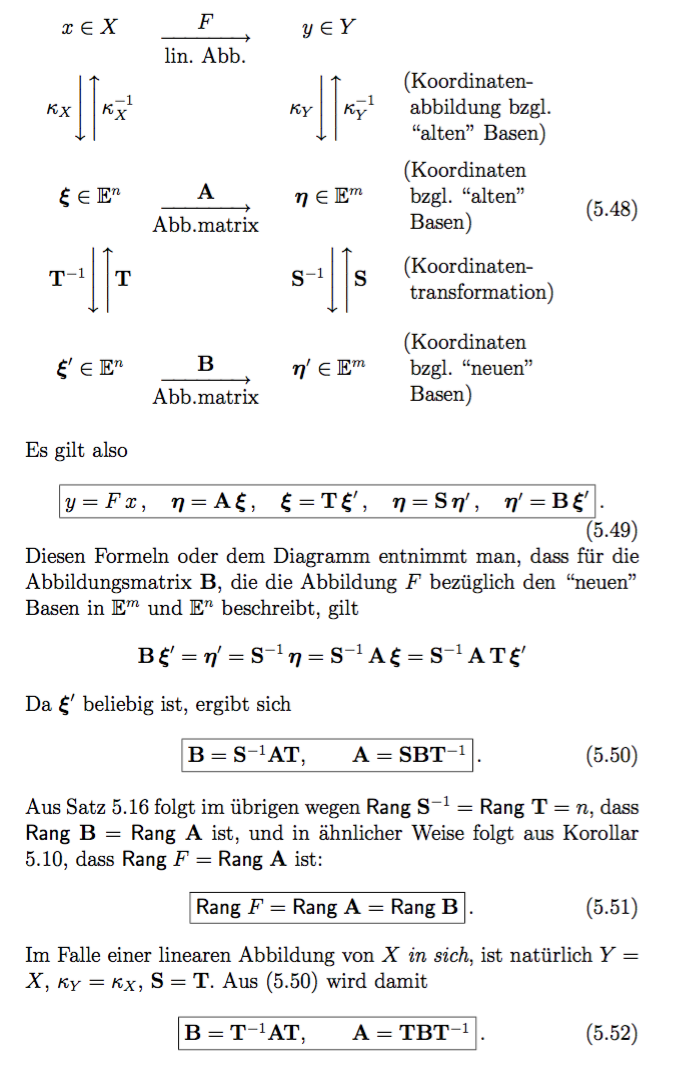
\includegraphics[width=400pt]{images/transformation}
\end{center}

\section{Projektionen}

\begin{description}[labelindent=16pt,style=multiline,leftmargin=5cm, noitemsep]
	\item[Projektion] lineare Abbildung f{\"u}r die gilt $P^2 = P$
	\item[Orthogonalprojektion]
	\begin{enumerate}
		\item Projektion f{\"u}r die gilt $\text{ker}\ P \perp \text{im}\ P$
		\item $P$ ist quadratisch
		\item $I-P$ ist orthogonaler Projektor
		\item $P^T = P$
	\end{enumerate}
\end{description}

\begin{equation*}
\begin{split}
	P_A & :\equiv A(A^HA)^{-1}A^H \\
	P_Q & :\equiv QQ^H\quad\text{falls Kolonnen von $Q$ orthonormal}
\end{split}
\end{equation*}

\subsection{Methode der kleinsten Quadrate}

Beispiel 7.4 Seite 7-7 im Skript

\subsection{QR-Zerlegung}

\begin{equation*}
\begin{split}
	\textbf{Grundsatz:} & \quad A = QR \\
	\text{mit} & \quad q_1 := \frac{a_1}{||a_1||},\ \tilde q_k := a_k - \sum_{j=1}^{k-1}q_j \langle q_j,\ a_k \rangle, q_k := \frac{\tilde q_k}{||\tilde q_k||} \\
	& \quad r_{11} :\equiv ||a_1||,\ r_{jk} :\equiv \langle q_j, a_k \rangle,\ r_{kk} :\equiv ||\tilde q_k||
\end{split}
\end{equation*}

\begin{equation*}
\begin{split}
	\text{gegeben:} & \quad A = \begin{pmatrix}
  1 & -1 & 4 \\
  1 & 4 & -2 \\
  1 & 4 & 2 \\
  1 & -1 & 0 
  \end{pmatrix} \\
	\text{Gram-Schmidt:} & \quad r_{11} = ||a_1||,\ q_1 = \frac{a_1}{||a_1||} = \frac{1}{2} \begin{pmatrix}1 \\ 1\\ 1\\ 1\end{pmatrix} \\
	& \quad r_{12} = q_1^T a_2 = \begin{pmatrix}\frac{1}{2} &\frac{1}{2} &\frac{1}{2} &\frac{1}{2}\end{pmatrix}\begin{pmatrix}-1\\4\\4\\-1\end{pmatrix} = 3 \\
	& \quad \tilde q_2 = (I - q_1q_1^T)a_2 = a_2 - r_{12}q_1 = \begin{pmatrix}-5/2 \\ 5/2 \\ 5/2 \\ -5/2\end{pmatrix} \\
	& \quad r_{22} = ||\tilde q_2 || = 5 \\
	& \quad q_2 = \frac{\tilde q_2}{||\tilde q_2||} = \begin{pmatrix}-1/2 \\ 1/2 \\ 1/2 \\ -1/2\end{pmatrix} \\
	& \quad \tilde q_3 = (I - q_1q_1^T)(I - q_2q_2^T)a_3 \\
	& \quad \text{und so weiter...} \\
	\textbf{L{\"o}sung:} & \quad Q = (q_1, q_2, q_3),\ R = \begin{pmatrix}
  r_{11} & r_{12} & r_{13} \\
  0 & r_{22} & r_{23} \\
  0 & 0 & r_{33} \\
  \end{pmatrix}
\end{split}
\end{equation*}

\section{Determinante}

Es gilt:
\begin{itemize}
	\item $\det A = 0 \Rightarrow Ax = b$ ist nicht l{\"o}sbar
	\item $A$ hat eine Zeile lauter Nullen $\Rightarrow \det A = 0$
	\item $A$ hat zwei gleiche Zeilen $\Rightarrow \det A = 0$
	\item $A$ ist eine Diagonalmatrix $\Rightarrow \det A =$ Produkt der Diagonalelemente
	\item $A$ ist eine Dreiecksmatrix $\Rightarrow \det A =$ Produkt der Diagonalelemente
\end{itemize}

\subsection{Identit{\"a}ten}

\begin{equation*}
\begin{split}
	\det(\gamma A)  & = \gamma^n \det A \\
	\det(AB) & = \det A \cdot \det B \\
	\det(A^{-1}) & = \det(A)^{-1} \quad\text{falls A regul{\"a}r} \\
	\det(A^T) & = \det(A) \\
	\det(A^H) & = \det(A)
\end{split}
\end{equation*}

\subsection{Berechnung}

\subsection{Dimension $2\times 2$}

\begin{equation*}
	\begin{vmatrix}
		a & b \\ c & d
	\end{vmatrix} = ad - cb
\end{equation*}

\subsection{Dimension $3\times 3$}

\begin{equation*}
	\begin{vmatrix}
		a & b & c \\ d & e & f \\ g & h & i
	\end{vmatrix} = (aei + dhc + gbf) - (gec + dbi + ahf)
\end{equation*}

\subsection{Allgemeine Dimension $n\times n$}

\begin{equation*}
\begin{split}
	\textbf{Grundsatz:}\quad & \det A = a_{kl} \mathcal{K}_{kl} \\
	\text{wobei} \quad & \mathcal{K}_{kl} :\equiv (-1)^{k+l} \det A_{[k,l]}
\end{split}
\end{equation*}

\emph{Tipp:} W{\"a}hle die Zeile/Spalte aus mit den meisten Nullen.

\begin{equation*}
\begin{split}
	\text{gegeben:} & \quad A = \begin{pmatrix}
		1 & 3 & 5 & 1 \\ 2 & 4 & 6 & 3 \\ 3 & 6 &4 & 2 \\1 & 5 & 3 & 1
	\end{pmatrix} \\
	\text{entwickeln nach der 2. Zeile:} & \quad \mathcal{K}_{21} = (-1)^3 \begin{vmatrix}
			3 & 5 & 1 \\ 6 &4 & 2 \\ 5 & 3 & 1
	\end{vmatrix} = -12 \\
	& \quad \mathcal{K}_{22} = (-1)^4 \begin{vmatrix}
			1 & 5 & 1 \\ 3 &4 & 2 \\ 1 & 3 & 1
	\end{vmatrix} = -2 \\
	& \quad \mathcal{K}_{23} = (-1)^5 \begin{vmatrix}
			1 & 3 & 1 \\ 3 &6 & 2 \\ 1 & 5 & 1
	\end{vmatrix} = -2 \\
	& \quad \mathcal{K}_{24} = (-1)^6 \begin{vmatrix}
			1 & 3 & 5 \\ 3 &6 & 4 \\ 1 & 5 & 3
	\end{vmatrix} = 28 \\
	\textbf{L{\"o}sung:} & \quad \det A = a_{21}\mathcal{K}_{21} + a_{22}\mathcal{K}_{22} + a_{23}\mathcal{K}_{23} + a_{24}\mathcal{K}_{24} \\
	& \quad =2(-12) + 4(-2) + 6(-2) + 3(28) = 40
\end{split}
\end{equation*}

\section{Eigenwerte und -vektoren}

Betrachte eine lineare Abbildung $F: V \mapsto V, x \mapsto Fx$:
\begin{description}[labelindent=16pt,style=multiline,leftmargin=3.5cm, noitemsep]
	\item[Eigenwert] $\lambda \in \mathbb{E}$, so dass $Fv = \lambda v$
	\item[Eigenvektor] $v \in V, v \neq 0$, so dass $Fv = \lambda v$
	\item[Eigenraum] geh{\"o}rt zu spezifischem Eigenwert $E_\lambda :\equiv \{v \in V; Fv = \lambda v\}$
	\item[Spektrum] $\sigma(F)$, Menge aller Eigenwerte von $F$
\end{description}

\subsection{Berechnung der Eigenwerte}

\begin{equation*}
	\textbf{Grundsatz:} \quad E_\lambda = \text{ker}\ (F - \lambda I) = \det(F - \lambda I)
\end{equation*}

\begin{equation*}
\begin{split}
	\text{gegeben:} & \quad A = \begin{pmatrix}
		5 & -1 & 3 \\ 8 & -1 & 6 \\ -4 & 1 & -2
	\end{pmatrix} \\
	\textbf{char. Polynom:} & \quad \det(A - \lambda I) = \begin{vmatrix}
		5 - \lambda & -1 & 3 \\ 8 & -1 - \lambda & 6 \\ -4 & 1 & -2-\lambda
	\end{vmatrix} = -\lambda(\lambda^2- 2\lambda+1) = \mathcal{X}_A(\lambda) \\
	\text{Nullstellen finden:} & \quad \lambda_1 = 1,\ \lambda_2 = 1,\ \lambda_3 = 0 \\
	\textbf{Eigenwerte:} & \quad \sigma(A) = \{1, 2, -1\}
\end{split}
\end{equation*}

\subsection{Berechnung der Eigenvektoren}

\textbf{Eigenwerte} in $A$ einsetzen

\begin{figure}[H]
    \centering
    \begin{minipage}{.5\textwidth}
        \begin{table}[H]
\centering
\begin{tabular}{|p{0.5cm}|p{0.5cm}|p{0.5cm}||p{0.5cm}|}
\hline
4  & -1 & 3  & 0 \\ \hline
8  & -2 & 6  & 0 \\ \hline
-4 & 1  & -3 & 0 \\ \hline
\end{tabular}
\end{table}
    \end{minipage}%
    \begin{minipage}{0.5\textwidth}
\begin{table}[H]
\centering
\begin{tabular}{|p{0.5cm}|p{0.5cm}|p{0.5cm}||p{0.5cm}|}
\hline
5  & -1 & 3  & 0 \\ \hline
8  & -1 & 6  & 0 \\ \hline
-4 & 1  & -2 & 0 \\ \hline
\end{tabular}
\end{table}
    \end{minipage}
\end{figure}

\begin{equation*}
	\Rightarrow v_1 = \begin{pmatrix}
		1 \\ 4 \\ 0
	\end{pmatrix},\ v_2 = \begin{pmatrix}
		0 \\ 3 \\ 1
	\end{pmatrix},\ v_3 = \begin{pmatrix}
		-1 \\ -2 \\ 1
	\end{pmatrix}
\end{equation*}

\subsection{Spektralzerlegung}

\begin{equation*}
	\textbf{Grundsatz:}\quad AV = V\Lambda \Leftrightarrow A = V\Lambda V^{-1}
\end{equation*}

\begin{equation*}
\begin{split}
	\text{gegeben:} \quad & A = \begin{pmatrix}
		-7 & 2 & -6 \\ 12 & -2 & 12 \\ 12 & -3 & 11
	\end{pmatrix} \\
	\text{Eigenwerte bestimmen:} \quad & \lambda_1 = 1,\ \lambda_2 = 2,\ \lambda_3 = -1 \\
	& \Rightarrow \Lambda = \begin{pmatrix}
		1 & 0 & 0 \\ 0 & 2 & 0 \\ 0 & 0 & -1
	\end{pmatrix} \\
	\text{Eigenvektoren bestimmen:} \quad & v_1 = \begin{pmatrix}
		1 \\ 4 \\ 0
	\end{pmatrix},\ v_2 = \begin{pmatrix}
		0 \\ 3 \\ 1
	\end{pmatrix},\ v_3 = \begin{pmatrix}
		-1 \\ 0 \\ 1
	\end{pmatrix} \\
	\textbf{Eigenbasis:} \quad & V = (v_1|v_2|v_3) = \begin{pmatrix}
		1 & 0 & -1 \\ 4 & 3 & 0 \\ 0 & 1 & 1
	\end{pmatrix}
\end{split}
\end{equation*}

\emph{Bemerkung:} $A$ muss diagonalisierbar sein, d.h. die \textbf{geometrische Vielfachheit} der Eigenwerte muss mit der \textbf{algebraischen Vielfachheit} {\"u}bereinstimmen.

\subsection{Hauptachsentransformation}

\begin{equation*}
\begin{split}
	\text{gegeben:} \quad & Q(x_1, x_2, x_3) = 221x_1^2 + 144x_1x_2 + 480x_1x_3 + 179x_2^2 + 360 x_2x_3 + 100x_3^2 \\
	\text{Matrix formen:} \quad & A = \begin{pmatrix}
		221 & 72 & 240 \\ 72 & 179 & 180 \\ 240 & 180 & 100
	\end{pmatrix} \\
	\textbf{Spektralzerlegung:} \quad & A = \begin{pmatrix}
		0.6 & 0.48 & 0.64 \\ -0.8 & 0.36 & 0.48 \\ 0 & -0.8 & 0.6
	\end{pmatrix} \begin{pmatrix}
		125 & 0 & 0 \\ 0 & -125 & 0 \\ 0 & 0 & 500
	\end{pmatrix} \begin{pmatrix}
		0.6 & -0.8 & 0 \\ 0.48 & 0.36 & -0.8 \\ 0.64 & 0.48 & 0.6
	\end{pmatrix} \\
	\text{neue Koordinaten:} \quad & \tilde x_1 = 0.6 x_1 - 0.8x_2 \\
	& \tilde x_2 = 0.48 x_1 + 0.36x_2 - 0.8x_3 \\
	& \tilde x_3 = 0.64x_1 + 0.48 x_2 + 0.6x_3 \\
	\textbf{Hauptachsendarstellung:} \quad & Q(x) = Q(\tilde x) = 125 \tilde x_1^2 -125\tilde x_2^2 + 500 \tilde x_3^2
\end{split}
\end{equation*}

\section{Singul{\"a}rwertzerlegung}

\begin{equation*}
\begin{split}
	\textbf{Grundsatz:}\quad & A = U\Sigma V^T \\
	\text{mit} \quad & \Sigma :\equiv \begin{pmatrix}
		\Sigma_r & 0 \\ 0 & 0
	\end{pmatrix},\ \Sigma_r = \text{diag}\{\sigma_1,...,\sigma_r\}, \text{wobei}\ \sigma_1 \geq \sigma_2 \geq ... \geq \sigma_r \\
	\text{wobei} \quad & \text{$\Sigma$ hat die gleiche Dimension wie $A$} \\
	& AA^T = U\Sigma^2_mU^T,\ A^TA = V\Sigma^2_nV^T \\
	& \text{$\{u_1,...,u_r\}$ ist Basis von $\text{im}\ A \equiv \mathcal{R}(A)$} \\
	& \text{$\{v_1,...,v_r\}$ ist Basis von $\text{im}\ A^T \equiv \mathcal{R}(A^T)$} \\
	& \text{$\{u_{r+1},...,u_m\}$ ist Basis von $\text{ker}\ A^H \equiv \mathcal{N}(A^H)$} \\
	& \text{$\{v_{r+1},...,v_n\}$ ist Basis von $\text{ker}\ A \equiv \mathcal{N}(A)$} \\
\end{split}
\end{equation*}

\begin{equation*}
\begin{split}
	\text{gegeben:}\quad & A = \begin{pmatrix}
		1 & 0 \\ 2 & 1 \\ 0 & 1
	\end{pmatrix} \\
	\text{$A^TA$ und $AA^T$ berechnen:}\quad & B = A^TA = \begin{pmatrix}
		5 & 2 \\ 2 & 2
	\end{pmatrix},\ C = AA^T = \begin{pmatrix}
		1 & 2 & 0 \\ 2 & 5 & 1 \\ 0 & 1 & 1
	\end{pmatrix} \\
	\textbf{Eigenwerte berechnen:} \quad & \sigma(B) = \{6, 1\},\ \sigma(C) = \{0, 1, 6\} \\
	\text{Grundsatz anwenden:} \quad & \Sigma = \begin{pmatrix}
		\sqrt{6} & 0 \\ 0 & \sqrt{1} \\ 0 & 0
	\end{pmatrix},\ \text{da}\ \sigma(B)\ \text{mit}\ |\sigma(B)| = 2\ \text{passt}\\
	\textbf{Eigenvektoren berechnen:} \quad & V = (b_1|b_2),\ U = (c_1|c_2|c_3) \\
	\text{}
\end{split}
\end{equation*}

\subsection{Spektralnorm}

\begin{equation*}
	||A||_2 = \sigma_1
\end{equation*}

\subsection{Konditionszahl}

\begin{equation*}
	\mathcal{K}(A) = ||A||_2\ ||A^{-1}||_2
\end{equation*}

Die Spektralnorm einer Matrix entspricht dem maximalen \textbf{Singul{\"a}rwert}.

\section{Differentialgleichungen}

\subsection{Erster Ordnung, homogen, linear, konstante Koeffizienten}

\begin{equation*}
\begin{split}
	\textbf{Grundsatz:}\quad & y(t) = Ve^{t\Lambda}c \\
	\text{mit}\quad & c = V^{-1}y_0
\end{split}
\end{equation*}

\begin{equation*}
\begin{split}
	\text{gegeben:} \quad & \dot y_1 (t) = -2y_1(t) + 2y_3(t) \\
	& \dot y_2(t) = -2y_1(t) - 3y_2(t) - 4y_3(t) \\
	& \dot y_3(t) = -3y_3(t) \\
	& y_1(0) = 0,\ y_2(0) = 0, y_3(0) = 1 \\
	\text{Matrix formen:} \quad & A = \begin{pmatrix}
		-2 & 0 & 2 \\ -2 & -3 & -4 \\ 0 & 0 & -3
	\end{pmatrix},\ y_0 = \begin{pmatrix} 0 \\ 0 \\ 1 \end{pmatrix} \\
	\textbf{Spektralzerlegung:}\quad & A = \begin{pmatrix}
		1 & -2 & 0 \\ -2 & 0 & -1 \\ 0 & 1 & 0
	\end{pmatrix}\begin{pmatrix}
		-2 & 0 & 0 \\ 0 & -3 & 0 \\ 0 & 0 & -3
	\end{pmatrix}\begin{pmatrix}
		1 & 0 & 2 \\ 0 & 0 & 1 \\ -2 & -1 & -4
	\end{pmatrix} \\
	\text{Grundsatz anwenden:}\quad & c = \begin{pmatrix}
		2 \\ 1 \\ -4
	\end{pmatrix} \\
	& y(t) = \begin{pmatrix}
		1 & -2 & 0 \\ -2 & 0 & -1 \\ 0 & 1 & 0
	\end{pmatrix} \begin{pmatrix}
		e^{-2t} & 0 & 0 \\ 0 & e^{-3t} & 0 \\ 0 & 0 & e^{-3t}
	\end{pmatrix}\begin{pmatrix}
		2 \\ 1 \\ -4
	\end{pmatrix} \\
	\textbf{L{\"o}sung:} \quad & y(t) = \begin{pmatrix}
		2e^{-2t}-2e^{-3t} \\ -4e^{-2t} + 4 e^{-3t} \\ e^{-3t}
	\end{pmatrix}
\end{split}
\end{equation*}

\subsection{H{\"o}here Ordnung, homogen, linear, konstante Koeffizienten}

\begin{center}
	\textbf{Grundsatz:} zu System 1. Ordnung umschreiben
\end{center}

\begin{equation*}
\begin{split}
	\text{gegeben:}\quad & \ddot x(t) - \dot x(t) -2x(t) = 0 \\
	& x(0) = 3,\ \dot x(0) = 0 \\
	\textbf{umformen:}\quad & y_1(t) = x(t),\ y_2(t) = \dot x(t) \\
	& \dot y_1 = y_2 \\
	& \dot y_2 = 2y_1 + y_2 \\
	& y_1(0) = 3,\ y_2(0) = 0 \\
	\text{Matrix formen:}\quad & A = \begin{pmatrix}
		0 & 1 \\ 2 & 1
	\end{pmatrix}, y_0 = \begin{pmatrix}
		3 \\ 0
	\end{pmatrix} \\
	\textbf{System 1. Ordnung l{\"o}sen:}\quad & y(t) = \begin{pmatrix}
		2e^{-t} & e^{2t} \\ -2e^{-t} & 2e^{2t}
	\end{pmatrix} \\
	\textbf{L{\"o}sung:} \quad & x(t) = x(t) = y_1(t) = 2e^{-t} + e^{2t}
\end{split}
\end{equation*}

\section{Maschinenzahlen}

\begin{equation*}
\begin{split}
	\text{gegeben:} \quad & x = \pm 0.bbb \times 2^{\pm bb} \\
	\textbf{gr{\"o}sste positive Zahl:} \quad & \frac{1}{2}+\frac{1}{4}+\frac{1}{8} = \frac{7}{8},\ \frac{7}{8} \times 2^3 = 7 \\
	\textbf{Maschinengenauigkeit:} \quad & 2^{-3} = \frac{1}{8} \\
\end{split}
\end{equation*}

\end{document}
